\chapter{Trials and Results}

\section{Lifetime separation, fixed $\tau_1$}

The aim of the first trial was to investigate how the separation between lifetime components affected the fit. PALS spectra containing two lifetime components were generated, corresponding to a two defect material in saturation trapping. The first lifetime, $\tau_1$, remained fixed at 180 ps while the second lifetime, $\tau_2$, decreased from 280 ps to 220 ps, in 10 ps intervals. 

For each pair of lifetimes, intensity was varied to simulate three diferent relative defect concentrations. The values chosen for the first lifetime intensity $I_1$ were 20\%, 50\% and 80\%, with $I_2 = 100\%-I_1$. 

Expectations were that:
\begin{enumerate}[label=(\roman*)]
    \item The overall fit would improve as lifetime separation, $\tau_1-\tau_2$, increases.
    \item The fit would improve for a given lifetime component as the intensity of that component increases.
\end{enumerate}

\begin{figure} [h]
     
    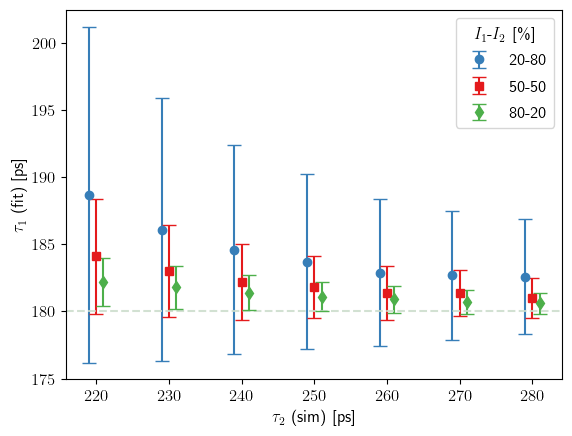
\includegraphics[width=0.6\linewidth]{Batch 1+2/Batch1+2/output/plotfin/t1.png}
    \caption{Fitted $\tau_1$}
    \label{fig:180-tau1}
\end{figure}

In Figure \ref{fig:180-tau1} is the fit for the first lifetime component $\tau_1$. As would be expected, the accuracy of the fit increases as both the separation between lifetimes and the intensity of $I_1$ increases. The size of the error bars indicates the precision of the fit, and seems to follow the same expected trend.

A similar picture emerges when looking at $\tau_2$, as can be seen in Figure \ref{fig:180-tau2}. Here, as the simulated value of $\tau_2$ that is being compared to the fitted $\tau_2$ is constantly changing, y-axis plots the difference between the two values. Nevertheless, we see that both accuracy and precision increase with lifetime separation and $I_2$ this time, which makes sense as the second lifetime is the observed variable.

In both cases, the fitted values of the component tend to be higher than their simulated counterparts. Outliers emerge when looking at the 80-20 data in the 220-240ps range, for both $\tau_1$ and $\tau_2$. This is harder to spot in the former, though, unless zoomed in (see Figure \ref{fig:180-tau1zoom}).

\vspace{0.5cm}
\begin{minipage}{.45\linewidth}
     
    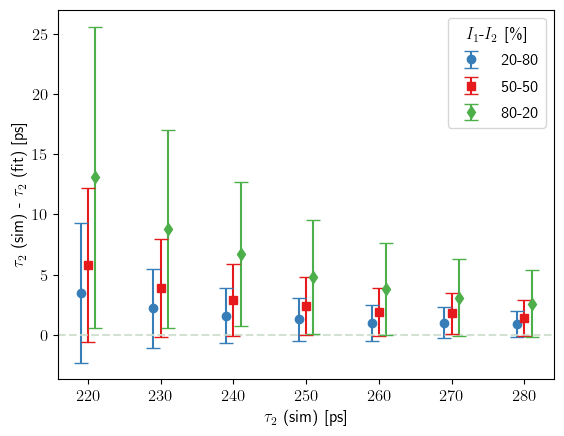
\includegraphics[width=\linewidth]{Batch 1+2/Batch1+2/output/plotfin/t2.png}
    \captionof{figure}{$\tau_2$ (Fitted$-$Simulated)}
    \label{fig:180-tau2}
\end{minipage}
\hfill
\begin{minipage}{.45\linewidth}
     
    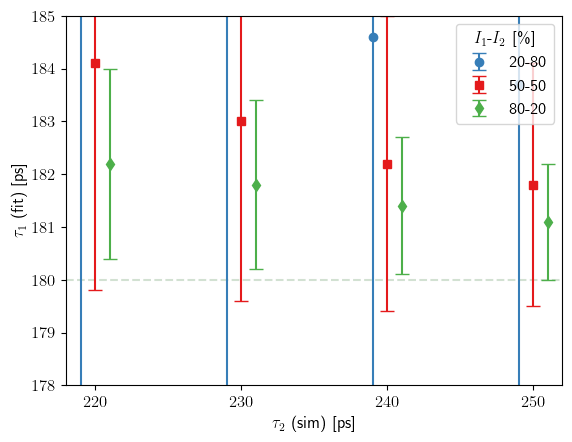
\includegraphics[width=\linewidth]{Batch 1+2/Batch1+2/output/plotfin/t1zoom.png}
    \captionof{figure}{Fitted $\tau_1$, $\tau_2 = [220-250]$}
    \label{fig:180-tau1zoom}
\end{minipage}
\vspace{0.5cm}

Plotting intensities (Figures \ref{fig:180-2080}, \ref{fig:180-5050} and \ref{fig:180-8020}), the same expected trends are observed. The error bars seem to get smaller, though, as the intensity of the first component $I_1$ increases. As a consequence, the error bars of the first three datapoints in Figure \ref{fig:180-8020} end up falling short of their simulated values.

\begin{minipage}{.45\linewidth}
    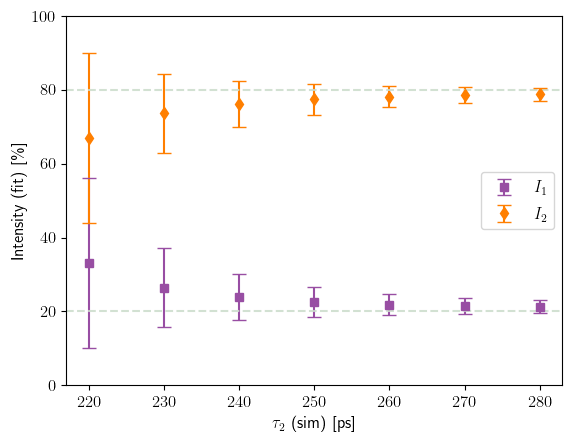
\includegraphics[width=\linewidth]{Batch 1+2/Batch1+2/output/plotfin/2080.png}
    \captionof{figure}{$I_1 = 20\%, I_2 = 80\%$}
    \label{fig:180-2080}
\end{minipage}
\hfill
\begin{minipage}{.45\linewidth}
    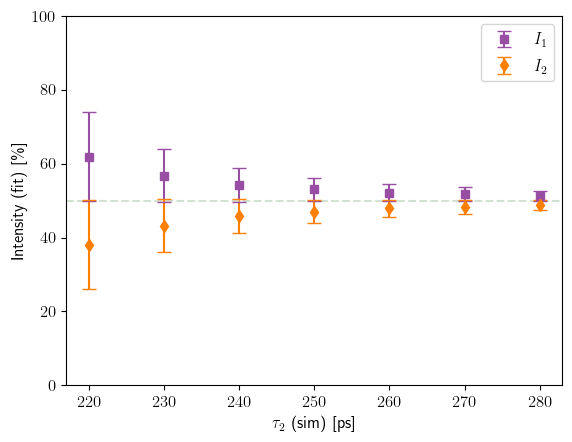
\includegraphics[width=\linewidth]{Batch 1+2/Batch1+2/output/plotfin/5050.png}
    \captionof{figure}{$I_1 = 50\%, I_2 = 50\%$}
    \label{fig:180-5050}
\end{minipage}
\begin{figure}[h]
    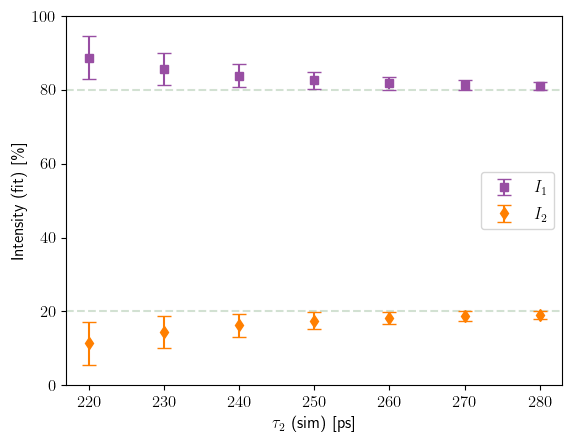
\includegraphics[width=0.45\linewidth]{Batch 1+2/Batch1+2/output/plotfin/8020.png}
    \caption{$I_1 = 80\%, I_2 = 20\%$}
    \label{fig:180-8020}
\end{figure}

\pagebreak

\section{Lifetime separation, varying $\tau_1$}

This trial builds on the previous, investigating the effect of varying $\tau_1$. Adding to the fits generated in the previous trial, two more sets of spectra were generated. 

In the first of these, every lifetime was shortened by 30ps. This meant that the first lifetime $\tau_1$ was set to 150ps and $\tau_2$ ranged from 190-250ps, while keeping the relative spacing consistent. The spectra were fitted, and the same plots generated in the previous trial were also generated for this set of spectra. The full set of plots are available in Appendix \ref{t1-150}.

The second set of spectra lengthened every lifetime by 40ps, so $\tau_1$ became 220ps and $\tau_2$ spanned 260-340ps. The same procedure was followed and the full set of plots are available in \ref{t1-220}. The $I_1$-$I_2$=20\%-80\%, $\tau_2=260ps$ spectrum is of interest, as the fit gives a highly inaccurate result with a very low standard deviation. This can be seen particularly well in Figure \ref{fig:220-t2-high}, and is notable in that, so far, a decrease in accuracy has always corresponded to a decrease in precision.

\vspace{0.5cm}

\begin{minipage}{.9\linewidth}
     
    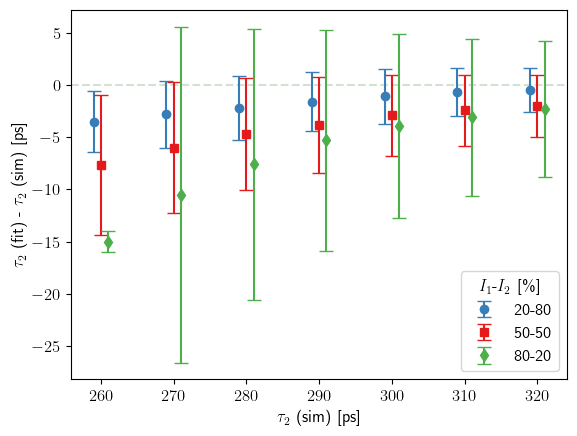
\includegraphics[width=0.6\linewidth]{Batch 3/regular IRF/tau1 220/output/plotfin/t2.png}
    \captionof{figure}{$\tau_2$ (Fitted$-$Simulated), $\tau_1=220$ps}
    \label{fig:220-t2-high}
\end{minipage}

\vspace{0.5cm}

Figure \ref{fig:220-t2-high} also shows an overall trend that is present in the lifetime fits for both the $\tau_1=220$ps and 150ps data. In both datasets, PALSfit tends to underestimate the lifetime fits, converging to the simulated values from the bottom. This is in contrast to the 180ps data (see Figures \ref{fig:180-tau1} and \ref{fig:180-tau2}), where the fits converged from the top. Other than that, trends in lifetime separation and component intensity are observed to be similar to the first trial.

Plots were generated to compare the three datasets, tracking both accuracy and precision. These can be found in Appendix \ref{comp-t1}. The odd bump in precision for the 80-20 spectrum mentioned earlier is clearly visible in the 80\%-20\% standard deviation plots (Figures \ref{fig:comp-t1err-8020}, \ref{fig:comp-t2err-8020} and \ref{fig:comp-Ierr-8020}). 

Overall though, while there is variation between the plots, the general trend seems to be that a decrease in $\tau_1$ corresponds to an improvement of the fit, as can be seen in Figure \ref{fig:comp-t2-ex}. In addition, the standard deviations for the 180ps and 150ps data tend to be closer to each other than to the 220ps data, a trend that doesn't seem as present in the fitted variables.

Comparing the two lifetime components, the fits for $\tau_2$ tend to be better overall than the $\tau_1$ fits. Looking at intensities, higher values for $I_1$ yields more accurate results, while standard deviation seems to be highest for the 50\%-50\% data.

\vspace{0.5cm}

\begin{minipage}{.9\linewidth}
     
    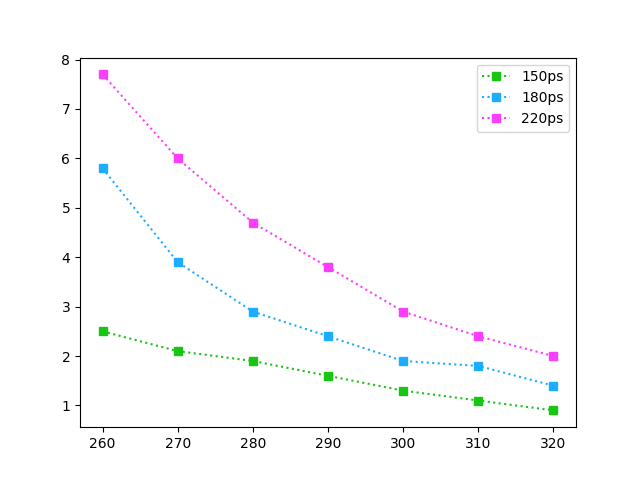
\includegraphics[width=0.6\linewidth]{Batch 3/regular IRF/t2-diff 5050.png}
    \captionof{figure}{$\tau_2$ (Fitted$-$Simulated)}
    \label{fig:comp-t2-ex}
\end{minipage}

\vspace{0.5cm}

\section{Resolution function width}

The aim of this trial was to investigate how the width of the resolution function affects the fit. While a narrower resolution function should result in a better fit, the idea was to quantify this improvement, as developing instrumentation that produce narrower resolution functions would require serious investment in time and resources.

As controlling the width of the resolution function is easier for a single Gaussian IRF, using the procedure outlined in \ref{singlegauss}, a 1-Gaussian approximation to the resolution function used in the previous trial was found. This resolution function was used to generate a series of spectra with fixed $\tau_1=150$ps and $\tau_2=180$-230ps. The results of the fit can be found in Appendix \ref{1g}. This was compared against the $\tau_1=150$ps fit from the last trial. The difference between the results of the two fits was deemed negligible.

Additional spectra were then generated and fitted using progressively narrower resolution functions, with FWHM = 180, 150 and 100. A comparison of the results is available in Appendix \ref{comp-irf}.

At a glance, an interesting pattern seems to emerge, based on the relative intensity of the components. When the intensity ratio $I_1$-$I_2$ = 20\%-80\% or 50\%-50\%, the narrower resolution functions produce the most accurate results (as in Figure \ref{fig:irf-reverse2080}). However, when the $I_1$-$I_2$ = 80\%-20\%, this trend seems to reverse (see Figure \ref{fig:irf-reverse8020}).

 

\begin{minipage}{.45\linewidth}
    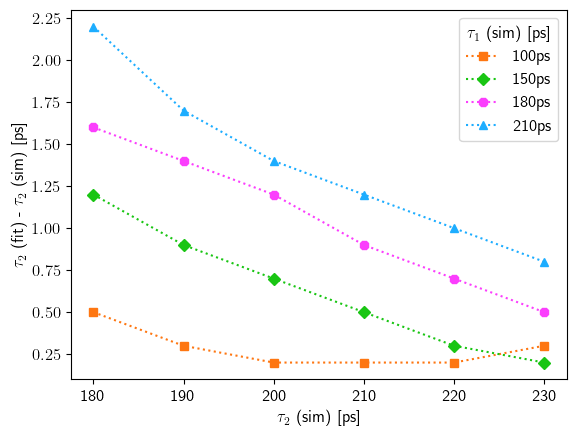
\includegraphics[width=.9\linewidth]{Batch 3/single Gaussian IRF/t2-diff 2080.png}
    \captionof{figure}{$I_1$-$I_2$=20\%-80\%}
    \label{fig:irf-reverse2080}
\end{minipage}
\hfill
\begin{minipage}{.45\linewidth}
    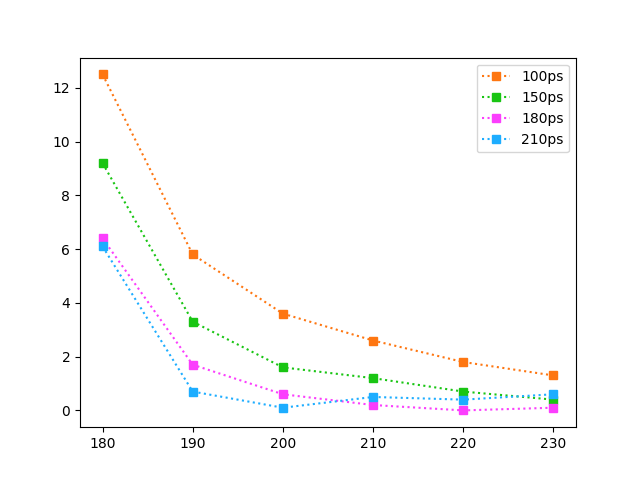
\includegraphics[width=.9\linewidth]{Batch 3/single Gaussian IRF/t2-diff 8020.png}
    \captionof{figure}{$I_1$-$I_2$=80\%-20\%}
    \label{fig:irf-reverse8020}
\end{minipage}

 

This reversal also occurs in some of the standard deviation plots, but the underlying pattern is less clear. The standard deviations do tend to quickly cluster together, though, as lifetime separation increases, indicating that the effect of the resolution function on the standard deviation is small.

Paying attention to the numbers, the overall effect of narrowing the resolution function is mixed, with the biggest improvements seen when fitting $\tau_1$ with $I_1$-$I_2$ = 20\%-80\% (Appendix \ref{fig:compirf-t1-2080}), and when fitting the intensities (Appendix \ref{fig:compirf-I-2080} and \ref{fig:compirf-I-5050}).

\section{Number of counts}

The goal of this trial is to examine how the total count number affects the fit. When generating spectra using PALSSIM, this is given as the area of the spectrum without the background and a separate background value. Both were kept constant in all previous trials, with the area set to $5.65 \times 10^6$ and the background value set to 8.5. Expectations were that a higher number of counts would make spectrum analysis easier. To test this hypothesis, spectra were generated with $\tau_1$ = 150ps, $\tau_2$ = 180-230ps and a 210ps FWHM single Gaussian resolution function, while tripling the background area to $1.7035 \times 10^7$. This allows for direct comparison with the data used in the previous trial, as a control.

Increasing the total area of the spectra and maintaining the same background value, however, increases the signal-to-noise ratio. As the easiest way to increase count number in practice is to increase experimental run-time, a more realistic scenario involves an equivalent increase in background noise. To model these, the same spectra were generated with both the tripled area and a proportional 3x increase in the background value (set to 25.5).

The generated spectra were then fitted with PALSFIT, and the results are summarized in Appendix \ref{comp-count}. Overall, increasing the total number of counts seemed to improve both the accuracy and the precision of the fits. As expected, this improvement was diminished when the background noise level was raised to match the increased count. In most cases though, the fit with the tripled count and the scaled background noise was much closer to the tripled count without background scaling than it was to the control, especially as lifetime separation increased. An example of this can be seen in Figure \ref{fig:thegood}.

 
\begin{minipage}{0.47\linewidth}
    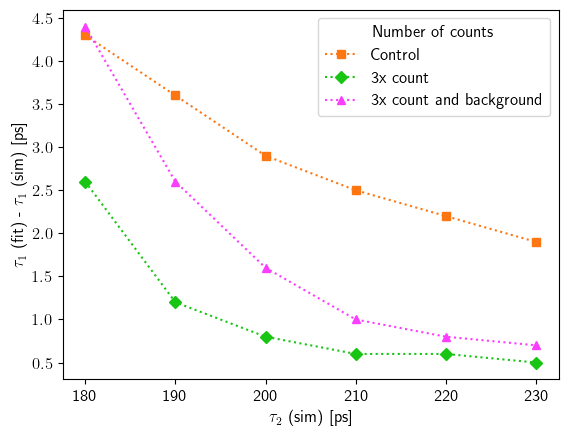
\includegraphics[width=\linewidth]{Batch 5/t1-diff 5050.png}
    \captionof{figure}{$\tau_2$, $I_1$-$I_2$ = 50\%-50\%}
    \label{fig:thegood}
\end{minipage}
\begin{minipage}{0.47\linewidth}
    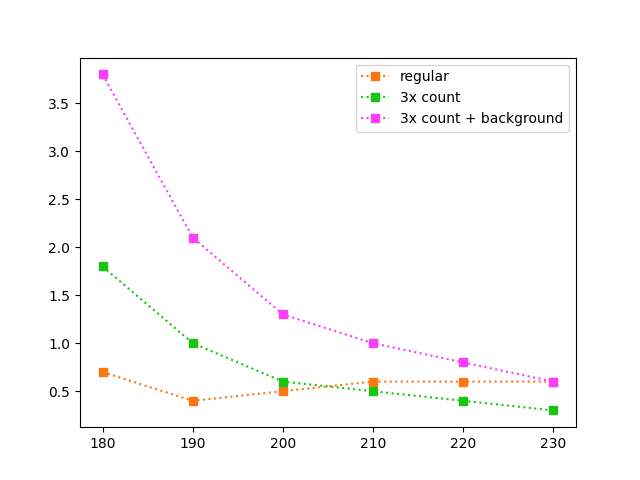
\includegraphics[width=\linewidth]{Batch 5/t1-diff 8020.png}
    \captionof{figure}{$\tau_2$, $I_1$-$I_2$ = 80\%-20\%}
    \label{fig:thebad}
\end{minipage}
 

Like in the last trial, though, the $I_1$-$I_2$ = 80\%-20\% fits show a reversal of the trend, as can be seen in Figure \ref{fig:thebad}. Unlike the previous trial, the reversal is not present in the standard deviations.


\section{Three lifetime components}

The goal of this trial was to model three-lifetime spectra, based on three experimental samples. The first two lifetimes would be defect lifetimes and the third was much longer and weaker than the former, characteristic of Para-Ps. During simulation, the third lifetime was kept constant at 2.6ns and an intensity of 0.15\%. The sample lifetimes are given in Table \ref{tab:3life}. 

\vspace{0.5cm}
\begin{minipage}{.35\linewidth}
     
    \captionof{table}{Lifetimes}
    \begin{tabular}{|c|c|c|}
        \hline
        $\tau_1$(ps) & $\tau_2$(ps) & $\tau_3$(ns)\\
        \hline
        370 & 442 & 2.6 \\
        355 & 444 & 2.6 \\
        348 & 440 & 2.6 \\
        \hline
    \end{tabular}
    \label{tab:3life}
\end{minipage}
\hfill
\begin{minipage}{.6\linewidth}
     
    \captionof{table}{Intensities}
    \begin{tabular}{|c|c|c|c|}
        \hline
        \multicolumn{2}{|c|}{relative} & \multicolumn{2}{|c|}{absolute} \\
        \hline
        $I_1$ & $I_2$ & $I_1$    & $I_2$   \\
        \hline
        99.5\% & 0.5\% & 99.3508\%   &  0.4993\%  \\
        90\%   & 10\%  & 89.865\%    &  9.985\%   \\
        80\%   & 20\%  & 89.88\%     & 19.97\%    \\
        50\%   & 50\%  & 49.925\%    & 49.925\%   \\
        20\%   & 80\%  & 19.97\%     &  9.985\%   \\
        \hline
    \end{tabular}
    \label{tab:relint}
\end{minipage}


The relative intensities between the first two lifetime components was varied, simulating different defect concentrations, as shown in Table \ref{tab:relint}. On the left side of the table are the relative intensities chosen. Due to the presence of the third component, the values for $I_1$ and $I_2$ had to be adjusted to those in the "absolute" column. To closer emulate the experimental process, each spectrum was fitted with one, two and then three components. The result of the fits can be found in Appendix \ref{3lifefits}.

The one-lifetime fits are found to roughly follow the average lifetime $\tau_{av}$. An example can be seen in Figure \ref{fig:1lifeex}. Of note is that PALSfit returns very small error bars. 

 
\begin{minipage}{.45\linewidth}
     
    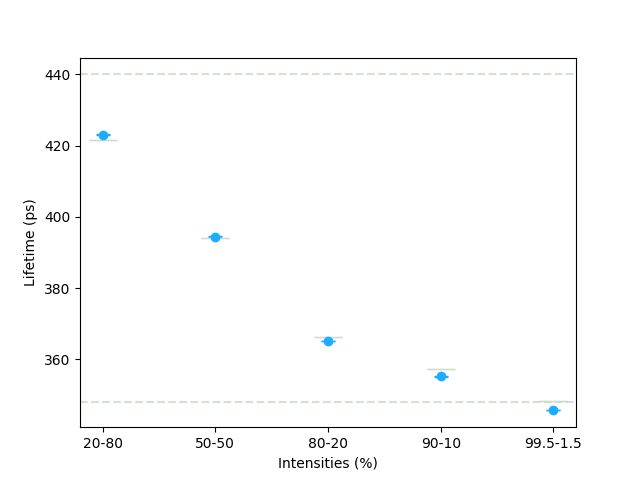
\includegraphics[width=\linewidth]{Batch 7/348-440/output/1 life/lifetime.png}    
    \captionof{figure}{One lifetime fit, $\tau_1=348$ps, $\tau_2=348$ps}
    \label{fig:1lifeex}
\end{minipage}
\hfill
\begin{minipage}{.45\linewidth}
     
    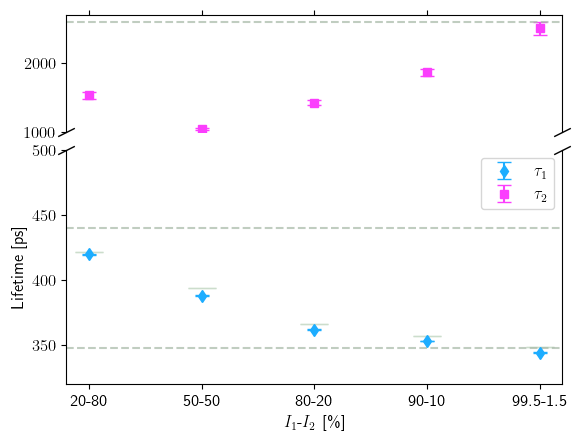
\includegraphics[width=\linewidth]{Batch 7/348-440/output/2 life/lifetimes.png}    
    \captionof{figure}{Two lifetime fit, $\tau_1=348$ps, $\tau_2=348$ps}
    \label{fig:2lifeex}
\end{minipage}
 

In the two-lifetime fits produced, the first component seems to follow $\tau_{av}$, and try to fit the Ps lifetime. This can be seen in Figure \ref{fig:2lifeex}. Looking at just the second component, we see that it trends closer to the simulated 2.6ns component as the difference between $I_1$ and $I_2$ grows. We can make sense of this physically as the three component spectrum trending closer to a two-component spectrum.

The intensity for the first lifetime is near-100\% and the second is near-0\%, as can be seen in the appendix. The tiny error bars seen in the one-lifetime fit also make a return, in both the intensity and lifetime plots.

 
\begin{minipage}{.45\linewidth}
     
    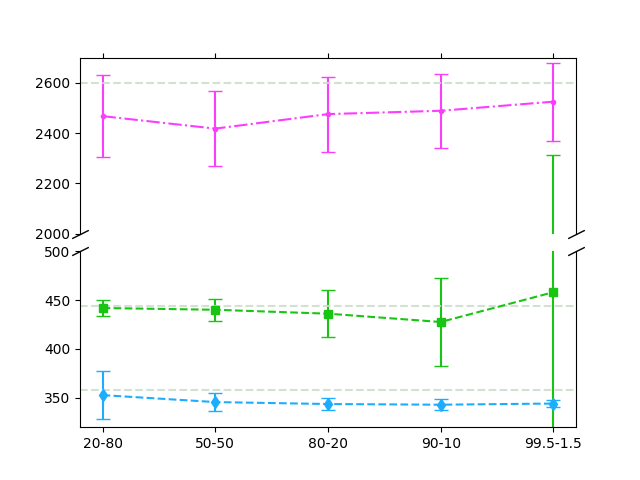
\includegraphics[width=\linewidth]{Batch 7/348-440/output/3 life/lifetimes.png}    
    \captionof{figure}{Three lifetime fit, $\tau_1=348$ps, $\tau_2=348$ps}
    \label{fig:3lifeex}
\end{minipage}
\hfill
\begin{minipage}{.45\linewidth}
     
    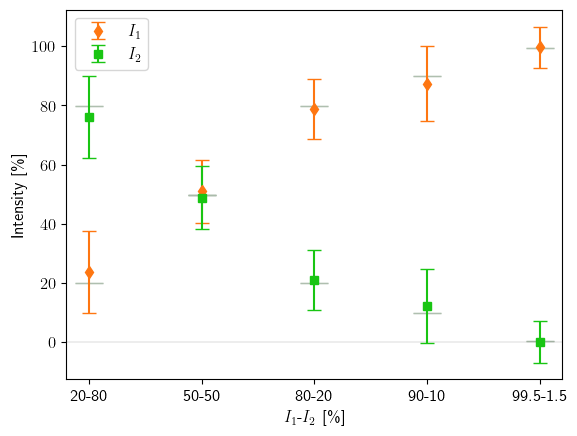
\includegraphics[width=\linewidth]{Batch 7/348-440/output/3 life/intensities.png}    
    \captionof{figure}{Intensities, three lifetime fit, $\tau_1=348$ps, $\tau_2=348$ps}
    \label{fig:3intex}
\end{minipage}
 

Finally, when looking at the three-lifetime fits, such as the ones shown in Figures \ref{fig:3lifeex} and \ref{fig:3intex}, the error bars come back and the three fitted components follow their simulated lifetime and intensity values. Datapoints where the fit fails are characterized by either massive or miniscule error bars, and tend to be concentrated towards the extremes, with regards to intensity. 

Additionally, the program seems to have a tendency to underestimate the third lifetime. Finally, as expected, the sample with the both the smallest lifetime separation and the longest first component ($\tau_1=370$ps and $\tau_1=370$ps) has the worst showing, overall.